\documentclass[a4paper,12pt]{article}
\usepackage{ctex}
\usepackage{amsmath}
\usepackage{graphicx}
\usepackage{geometry}
\usepackage{diagbox}
\usepackage{multirow}
\usepackage{hyperref}
\usepackage{float}
\usepackage{tikz}
\usepackage{subcaption}
\usepackage{csvsimple}
\usepackage{array}
\usepackage{tabularx}
\usetikzlibrary{arrows.meta,positioning}
\newcolumntype{Y}{>{\centering\arraybackslash}X}
\geometry{left=2.5cm,right=2.5cm,top=2.5cm,bottom=2.5cm}
\graphicspath{{figures/}{results/}}

\begin{document}
\begin{titlepage}
    \centering
    \vfill
    {\zihao{0}\bfseries 电子测试与实验技术\\[0.6em]实验报告\par}
    \vfill
    \vfill

    \begin{minipage}{0.72\textwidth}
        \zihao{-2}
        学\quad\quad 院：\underline{\makebox[7.5cm][l]{光学与电子信息学院}}\\[1.6em]
        班\quad\quad 级：\underline{\makebox[7.5cm][l]{光电信息科学与工程202409班}}\\[1.6em]
        姓\quad\quad 名：\underline{\makebox[7.5cm][l]{陈\quad 恪\quad 瑾}}\\[1.6em]
        学\quad\quad 号：\underline{\makebox[7.5cm][l]{U 2 0 2 4 1 3 9 2 5}}\\[1.6em]
        实验时间：\underline{\makebox[7.5cm][l]{2026 年 06 月 04 日}}
    \end{minipage}

    \vfill
    \vfill
\end{titlepage}

\setcounter{page}{1}

\section{实验名称}
计数译码显示电路与数字钟设计

\section{实验目的}
\begin{enumerate}
    \item 掌握中规模集成计数器 CC40161（实验中对应 74HC161）的逻辑功能与使用方法。
    \item 掌握计数、译码、显示电路的实现与调试方法。
    \item 完成简易数字钟（时、分计数）的搭建与功能验证。
\end{enumerate}

\section{实验元器件}
\begin{table}[H]
\centering
\caption{实验元器件清单}
\begin{tabular}{|c|c|c|}
\hline
类型 & 型号（参数） & 数量 \\
\hline
集成电路 & CD4511 & 4片 \\
\hline
集成电路 & 74HC161 & 4片 \\
\hline
集成电路 & 74HC00 & 4片 \\
\hline
数码管 & 5161AS & 4只 \\
\hline
\end{tabular}
\end{table}

\section{预习要求}
\begin{enumerate}
    \item 复习七段译码器译码、共阴极显示器，理解计数、译码与显示电路工作原理。
    \item 查阅相关芯片引脚图，熟悉逻辑功能与使用方法。
\end{enumerate}

\section{实验原理及参考电路}
\subsection{实验原理}
通过计数器对 1Hz 的时钟信号进行计数，并利用置位与清零功能产生进位，构成符合时间进制的计数电路。计数输出送入七段译码器后，译码器输出七位控制信号驱动数码管显示，从而实现简易时钟。

\subsection{参考电路}
\begin{figure}[H]
    \centering
    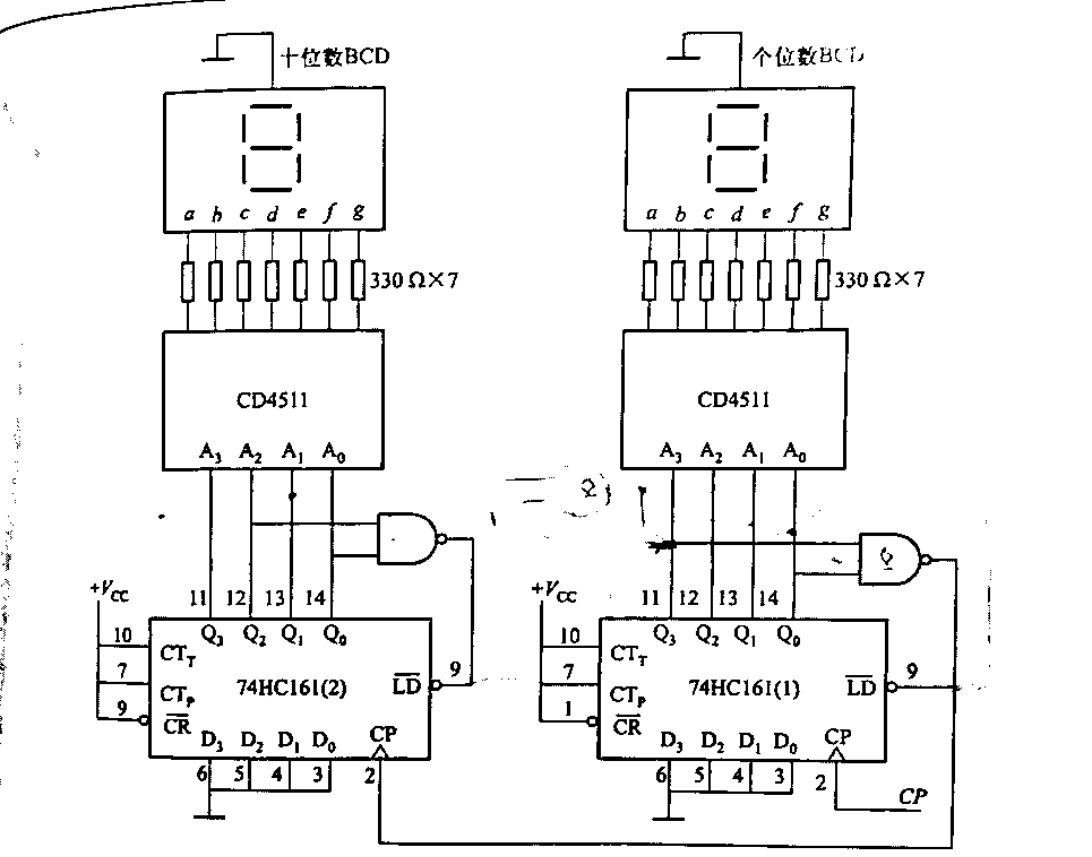
\includegraphics[width=0.62\textwidth]{figures/references/image1.png}
    \caption{0$\sim$59 同步计数参考电路}
\end{figure}

如图所示为 0$\sim$59 计数器（BCD 码）参考方案。当低位计数器输出到 1001 时产生置位信号，在下一个时钟沿到来时回到 0000，同时向高位计数器产生进位；当高位到 0101 且低位到 1001 时，下个时钟沿同时回零，实现 59 到 00 的同步翻转。采用类似方法可扩展构成 24 进制计数。

\section{硬件实验内容}
\subsection{设计过程}
\subsubsection{数码管显示}
每位数码管由一个 CD4511 译码器控制，输入为 4 位二进制计数（用74HC161输出）输出，输出为 7 位控制信号驱动数码管显示对应的十进制数字。通过调整译码器输入与数码管连接方式，确保正确显示 0$\sim$9 的数字。

具体来说，数码管的 a$\sim$g 七段分别连接到 CD4511 的 a$\sim$g 输出端，CD4511 的输入端连接到 74HC161 的输出 $Q_3,Q_2,Q_1,Q_0$，实现二进制到七段显示的译码功能，CD4511 的 LT、LE端低电平，BI 端接高电平，确保数码管正常显示状态。

数码管显示电路原理图如下：
\begin{figure}[H]
    \centering
    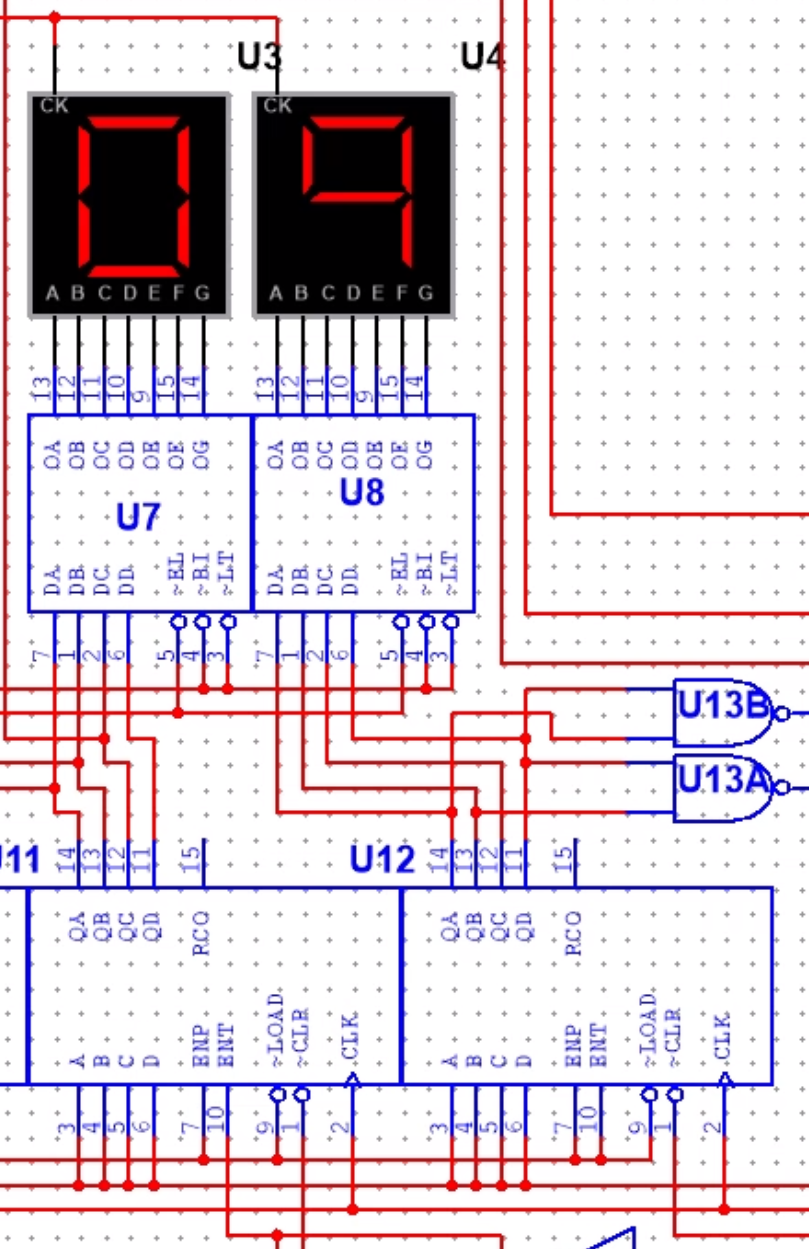
\includegraphics[width=0.86\textwidth]{figures/eda/image1.png}
    \caption{数码管显示电路原理图}
\end{figure}

\subsubsection{分计时}
先分别设计模 10 与模 6 计数器，再进行级联得到模 60 计数器实现分钟计时。

具体来说，分钟个位计数器由一个 $74HC161$ 构成，采用模 10 计数。利用其异步清零功能，当个位计数到 ${1010}_{2}({10}_{10})$ 时通过 $74HC00$ 的与非门产生低电平信号，连接到 $74HC161$ 的 $CLR$ 引脚实现清零，其逻辑式为
\[
CLR_U=\overline{M_{U3}\cdot \overline{M_{U2}}\cdot M_{U1}\cdot \overline{M_{U0}}}
\]
其中 $M_{U3},M_{U2},M_{U1},M_{U0}$ 为分钟个位计数器的输出。

分钟十位计数器由另一个 $74HC161$ 构成，采用模 6 计数。利用其异步清零功能，当十位计数到 ${0110}_{2}({6}_{10})$ 时，通过门电路译码产生低电平清零信号，接到 $74HC161$ 的 $CLR$ 引脚，使计数器立即清零回到 $0000$，从而实现 $0\sim5$ 的循环计数，其逻辑式为
\[
CLR_T=\overline{\overline{M_{T3}}\cdot M_{T2}\cdot M_{T1}\cdot \overline{M_{T0}}}
\]
其中 $M_{T3},M_{T2},M_{T1},M_{T0}$ 为分钟十位计数器的输出。

当分钟个位计数器计数到 $1001_2(9_{10})$ 时，产生进位信号连接到分钟十位计数器的 $ENT(ENP)$ 引脚，使分钟十位计数器在下一个 $CLK$ 的上升沿加 1，保证分钟部分的正确进位，其逻辑式为
\[
C_U=M_{U3}\cdot \overline{M_{U2}}\cdot \overline{M_{U1}}\cdot M_{U0}
\]

通过模 10 与模 6 计数器级联连接，即可形成分钟部分的模 60 计数器，其原理图如下：
\begin{figure}[H]
    \centering
    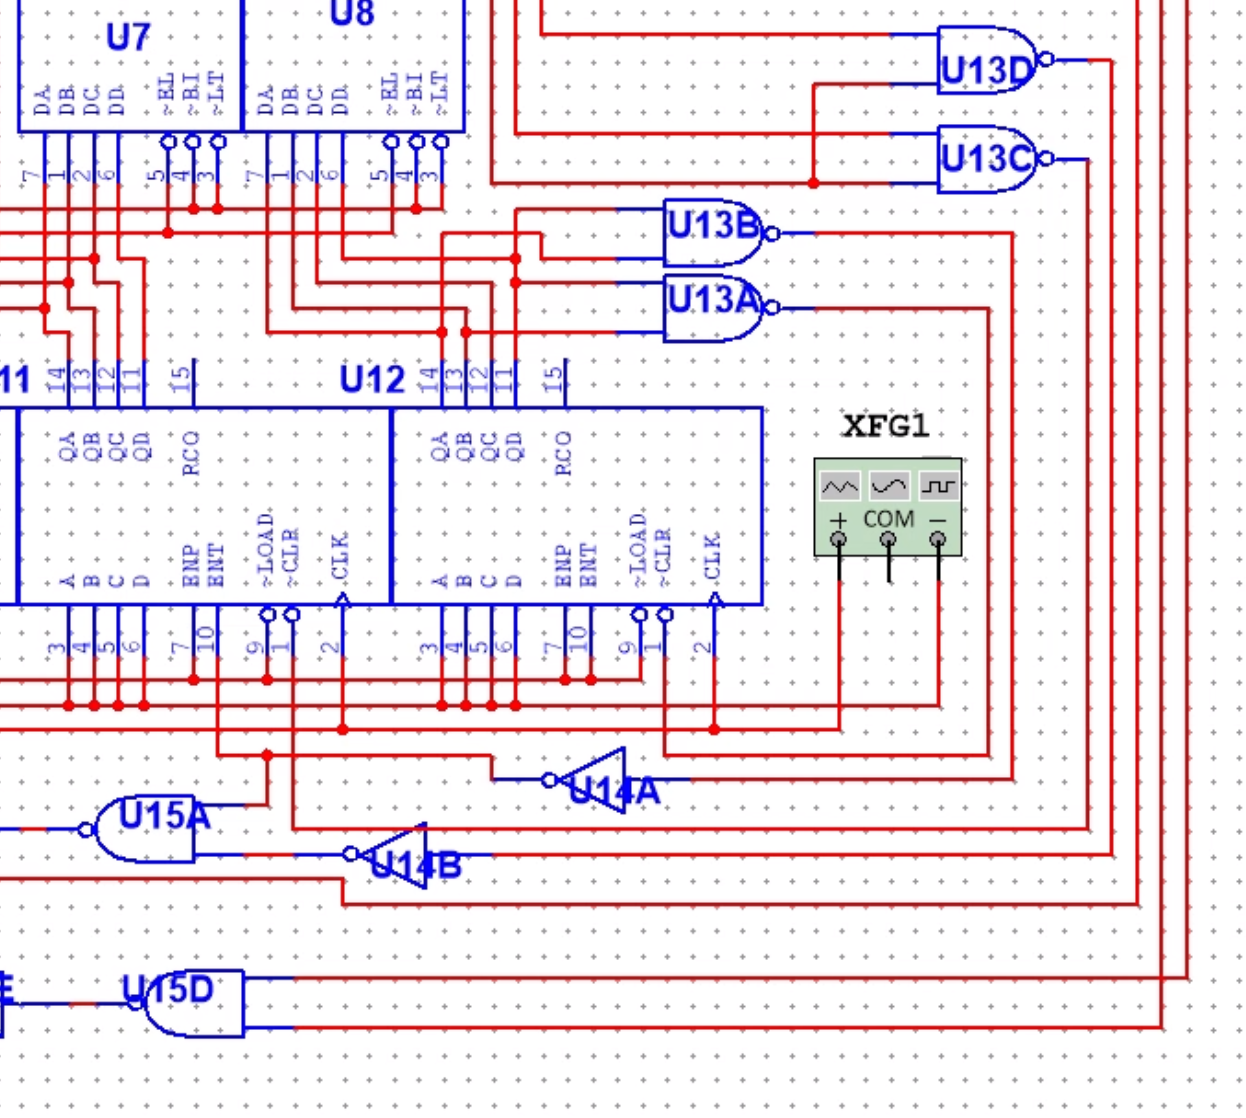
\includegraphics[width=0.86\textwidth]{figures/eda/image2.png}
    \caption{分钟计数电路原理图}
\end{figure}

\subsubsection{时计时}
采用相同的级联思路完成小时部分。小时计数器由两个 $74HC161$ 构成，分别作为小时个位计数器和小时十位计数器，其中小时个位采用 BCD 计数方式。分钟部分由 $59$ 翻转到 $00$ 时产生的进位信号作为小时部分的计数使能信号，使小时计数器只在每小时结束时加 $1$，其逻辑式为
\[
C_M=\overline{M_{T3}}\cdot M_{T2}\cdot \overline{M_{T1}}\cdot M_{T0}\cdot
M_{U3}\cdot \overline{M_{U2}}\cdot \overline{M_{U1}}\cdot M_{U0}
\]
其中 $M_{T3},M_{T2},M_{T1},M_{T0}$ 为分钟十位计数器输出，$M_{U3},M_{U2},M_{U1},M_{U0}$ 为分钟个位计数器输出。

当小时个位计数器计数到 $1001_2(9_{10})$ 且分钟部分产生进位时，向小时十位计数器产生进位信号，使小时显示由 $09$ 进入 $10$，其逻辑式为
\[
ENT_T=C_M\cdot U_3\cdot \overline{U_2}\cdot \overline{U_1}\cdot U_0
\]
其中 $C_M$ 为分钟部分的进位信号，$U_3,U_2,U_1,U_0$ 为小时个位计数器的输出。

为实现 $12$ 小时制，当小时显示为 $12$ 且分钟部分再次产生进位时，应使小时部分在下一个 $CLK$ 上升沿同步置数为 $01$。此时小时十位为 $0001_2$，小时个位为 $0010_2$，因此可通过门电路产生低电平置数信号，分别连接到两个 $74HC161$ 的 $LOAD$ 引脚，其逻辑式为
\[
LOAD_H=\overline{C_M\cdot \overline{T_3}\cdot \overline{T_2}\cdot \overline{T_1}\cdot T_0\cdot
\overline{U_3}\cdot \overline{U_2}\cdot U_1\cdot \overline{U_0}}
\]
其中 $T_3,T_2,T_1,T_0$ 为小时十位计数器的输出。将小时十位计数器的数据输入端预置为 $0000$，小时个位计数器的数据输入端预置为 $0001$，即可使电路在 $12$ 时 $59$ 分后的下一个时钟周期回到 $01$ 时 $00$ 分。

具体电路原理图如下：
\begin{figure}[H]
    \centering
    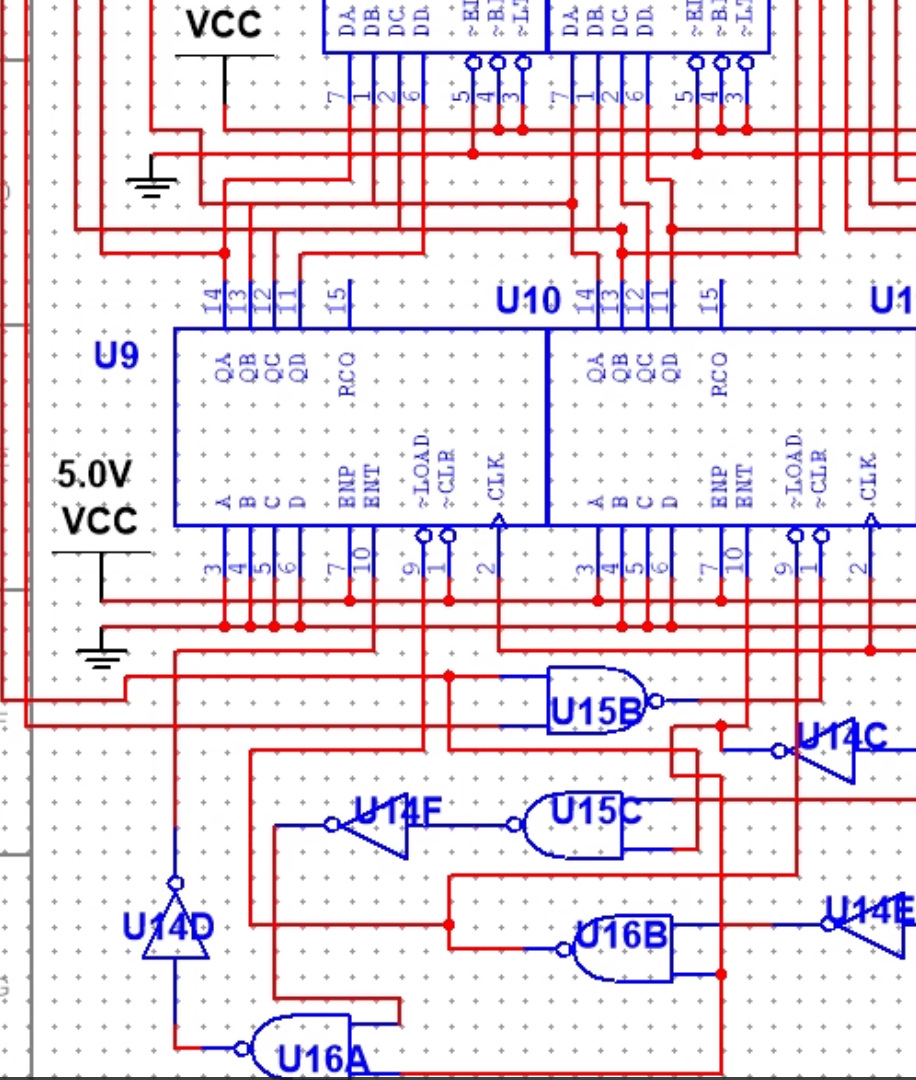
\includegraphics[width=0.86\textwidth]{figures/eda/image3.png}
    \caption{小时计数电路原理图}   
\end{figure}

\subsection{电路原理图}
将上述设计的数码管显示电路、分钟计数电路与小时计数电路进行连接，得到完整的数字时钟电路原理图如下：
\begin{figure}[H]
    \centering
    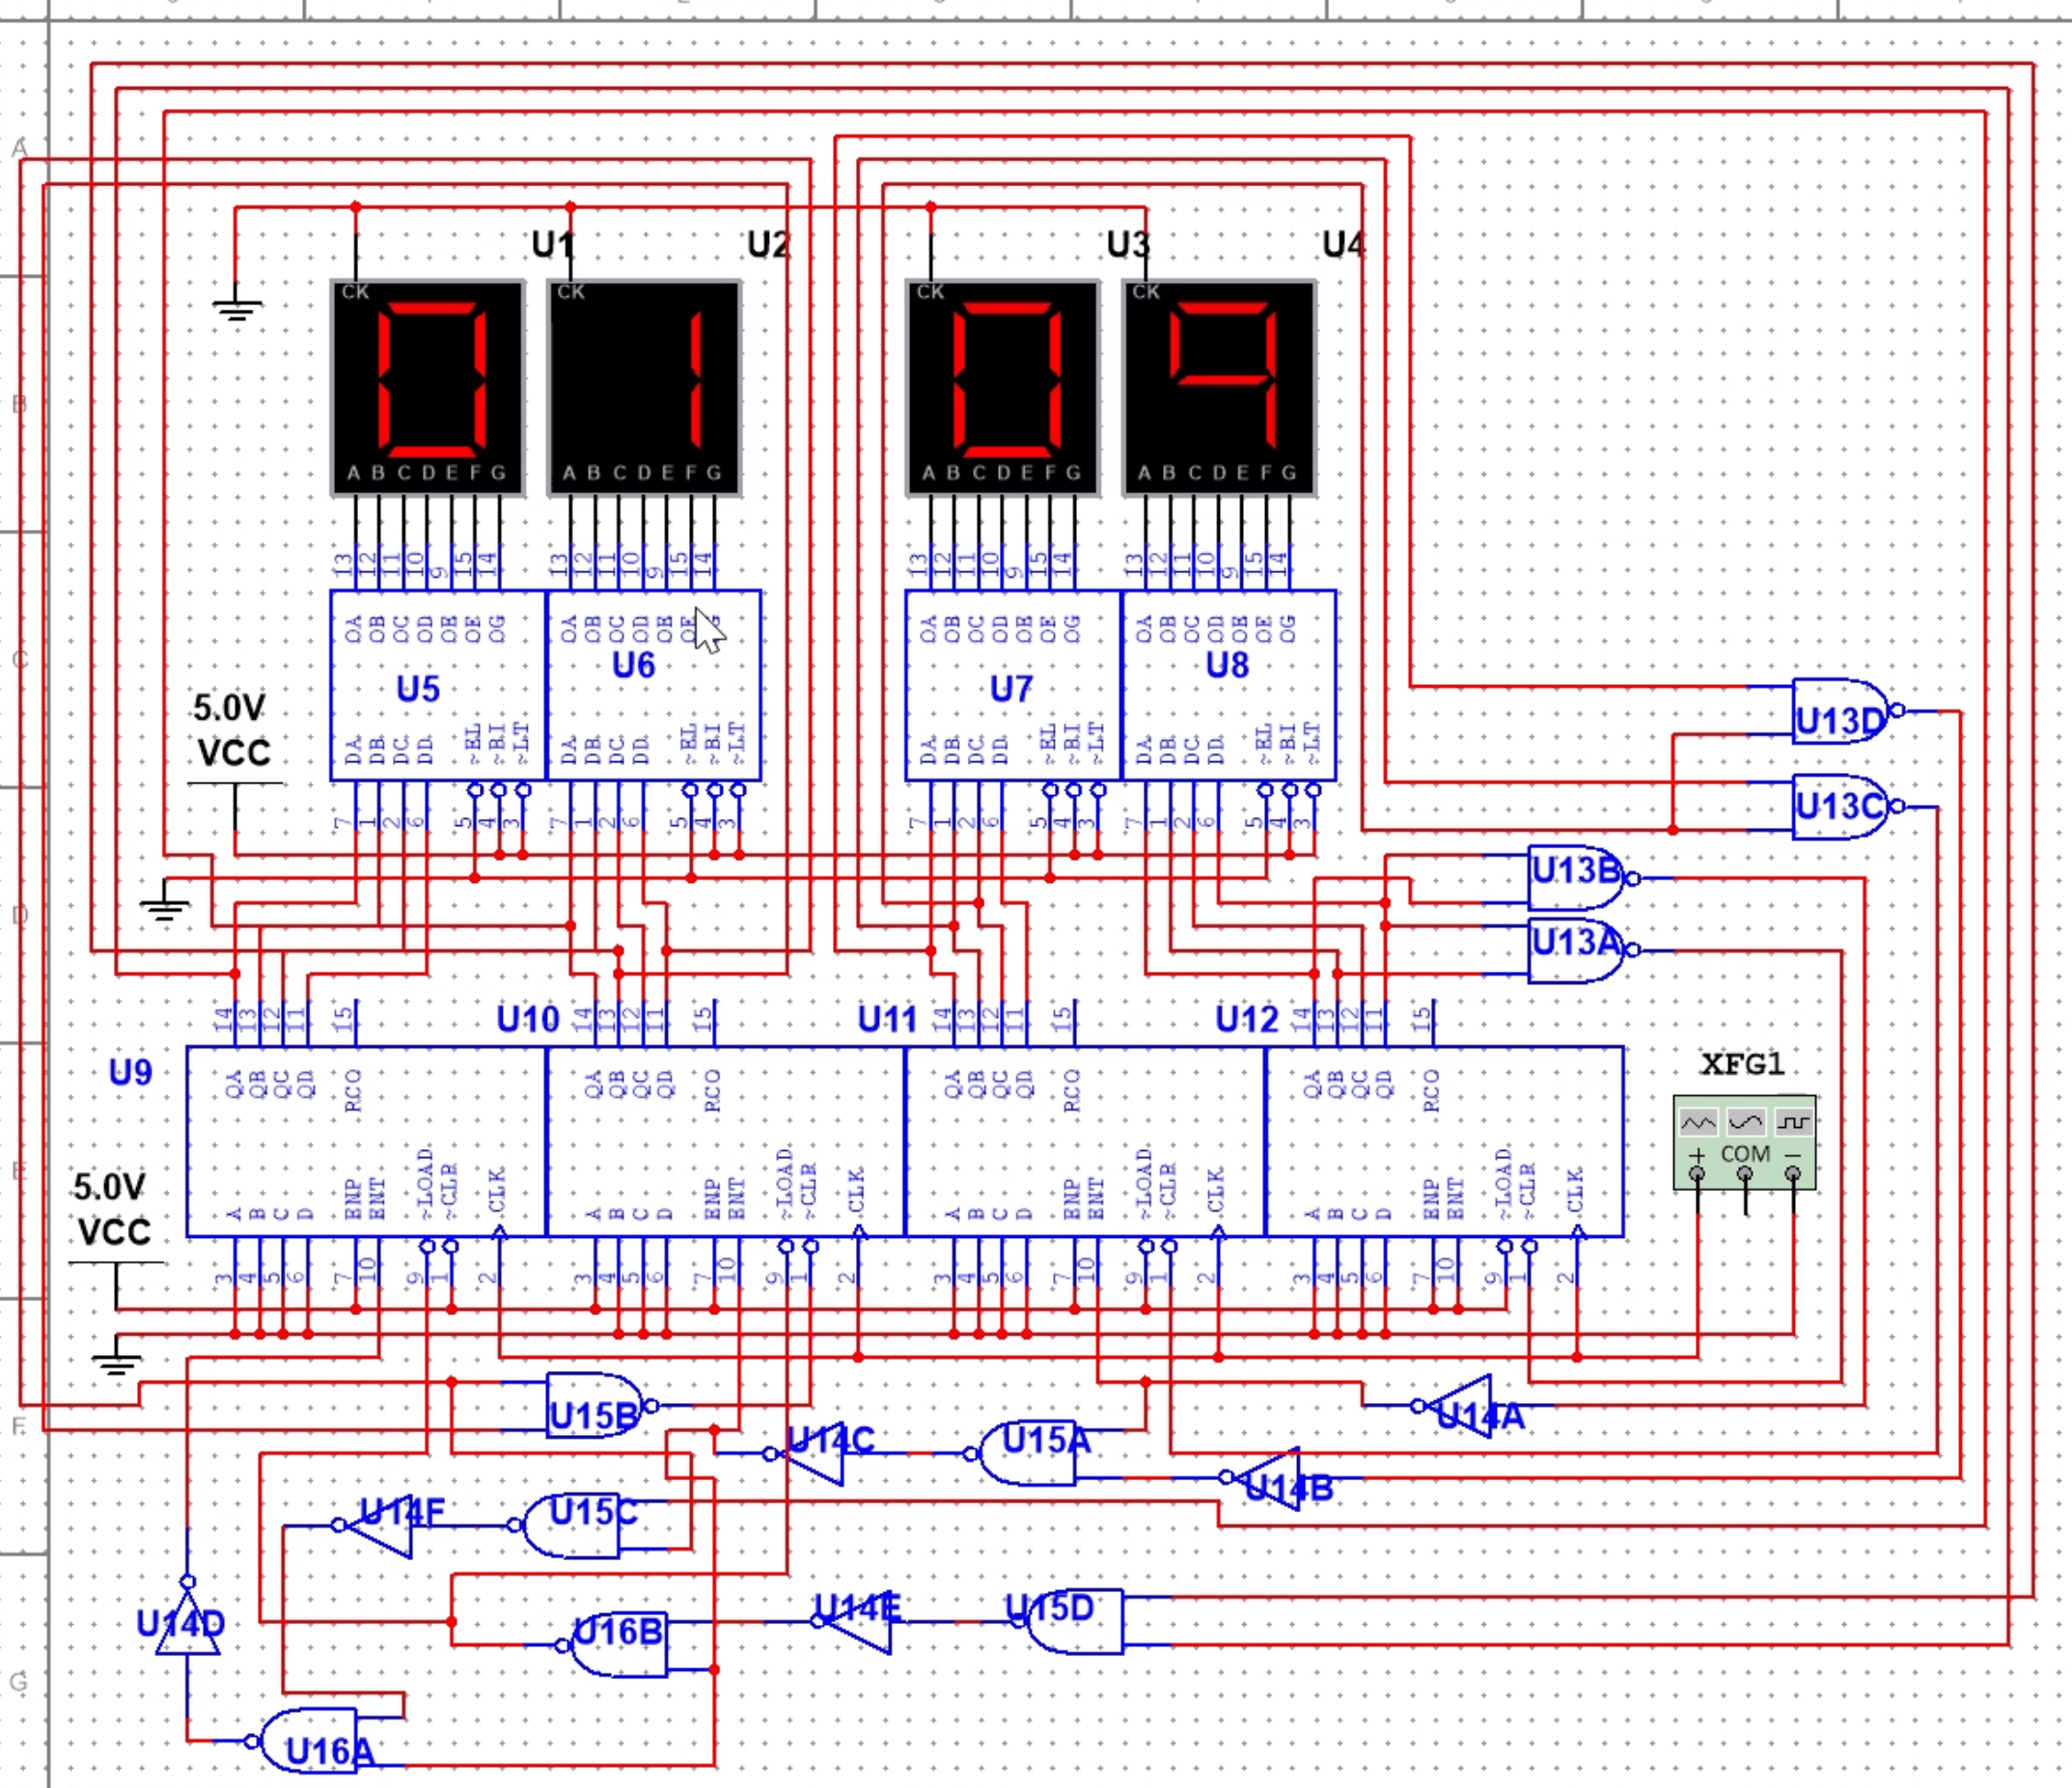
\includegraphics[width=0.86\textwidth]{figures/eda/image4.png}
    \caption{数字时钟电路原理图}
\end{figure}

\subsection{电路仿真结果}
使用 Multisim 软件对设计的数字时钟电路进行仿真，输入 1Hz 的时钟信号，观察数码管显示的分钟和小时部分是否正确计数和翻转。仿真结果如下：
\begin{figure}[H]
    \centering
    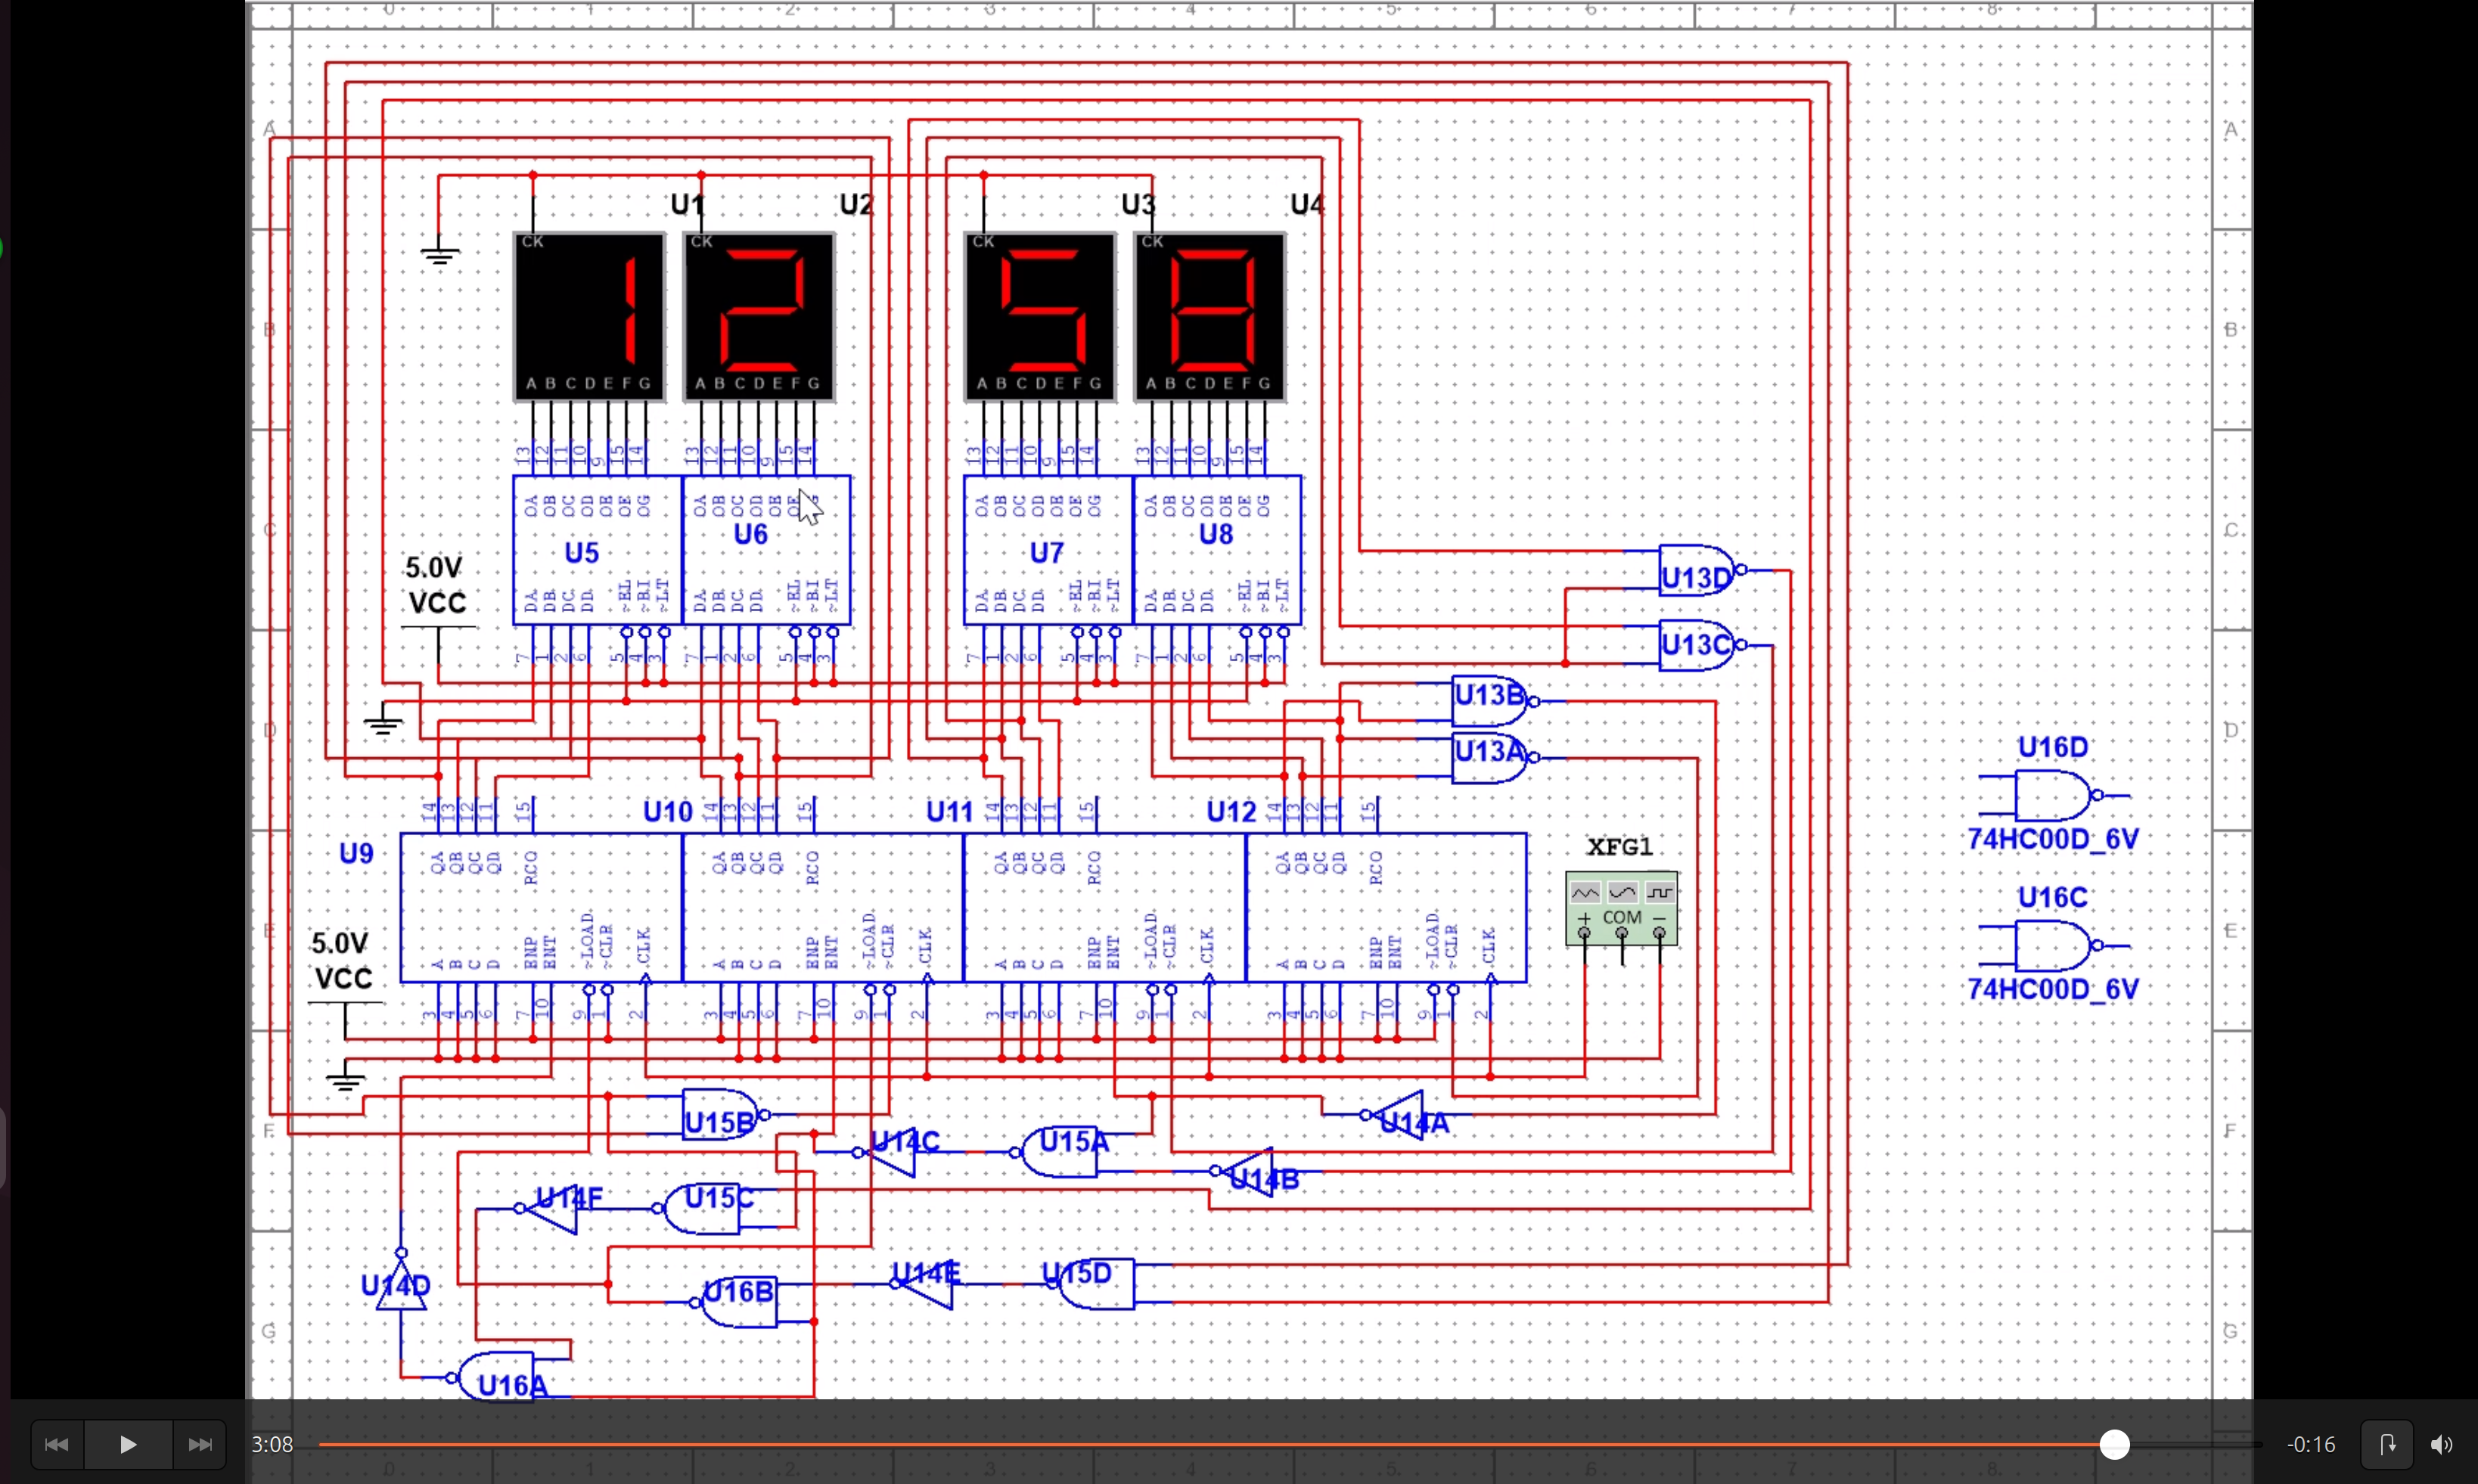
\includegraphics[width=0.86\textwidth]{figures/eda/image5.png}
    \caption{12时58分}
\end{figure}
\begin{figure}[H]
    \centering
    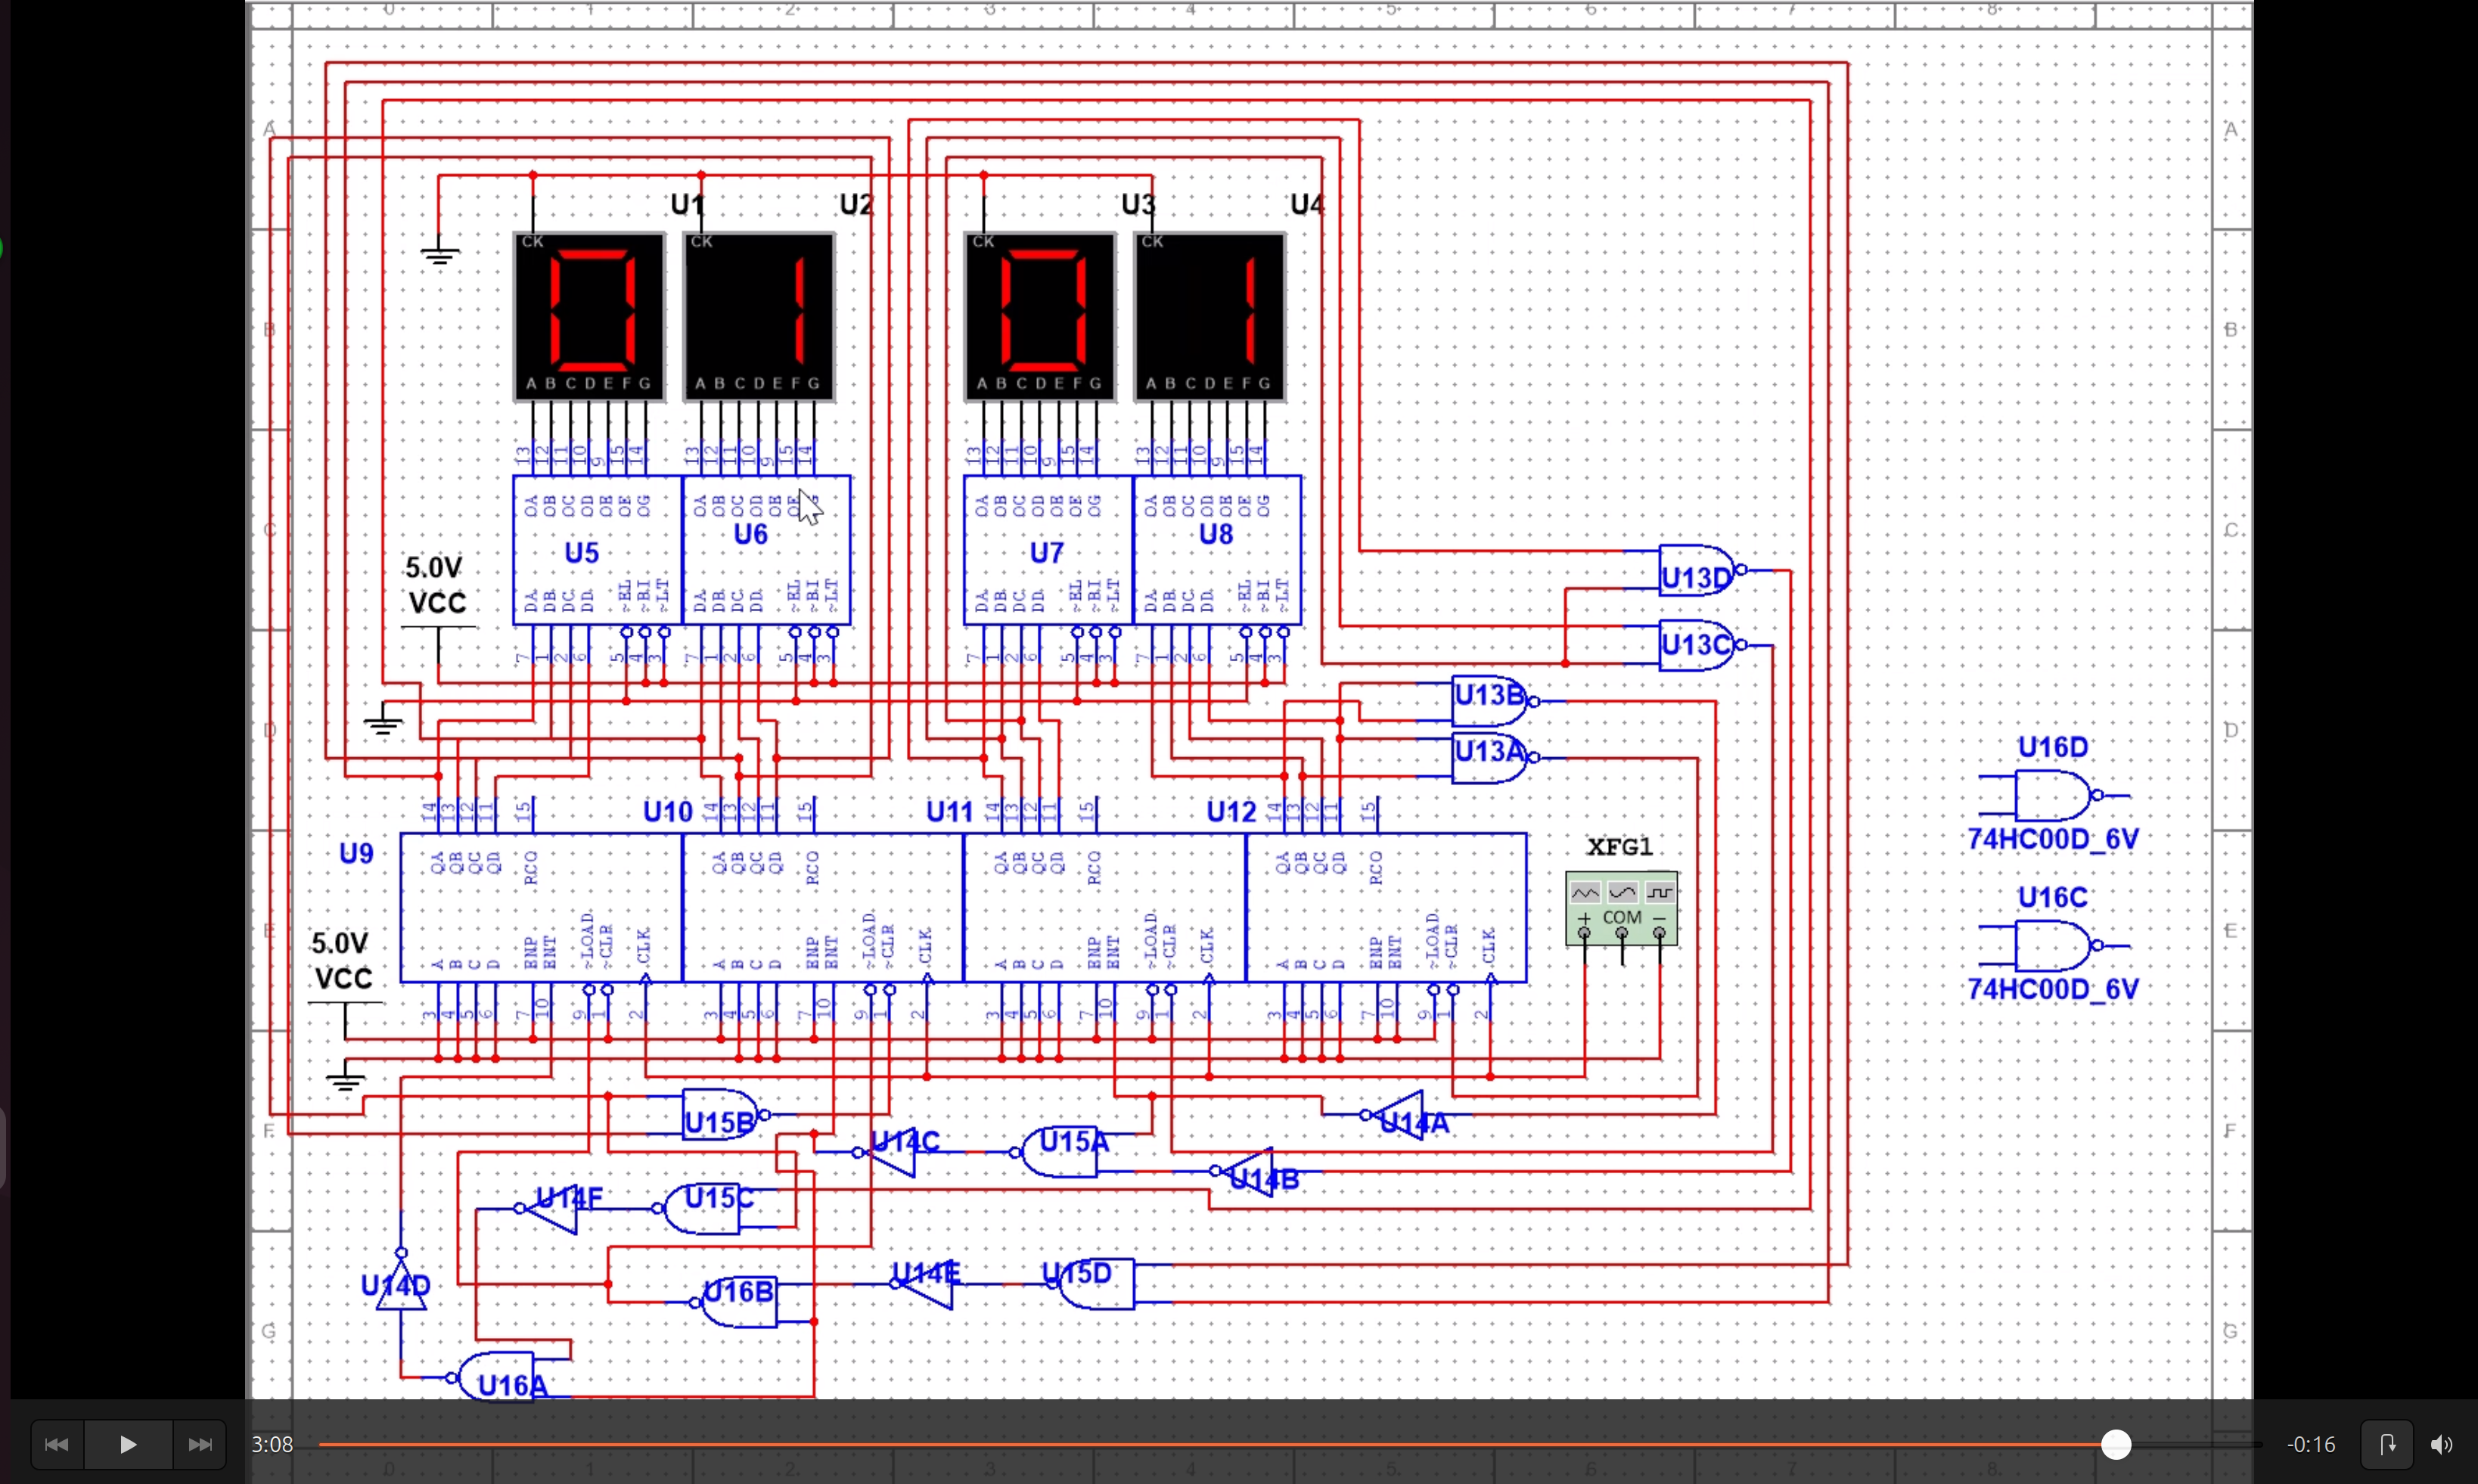
\includegraphics[width=0.86\textwidth]{figures/eda/image6.png}
    \caption{01时01分}
\end{figure}
仿真结果显示，时钟处于12时59分后，分钟部分正确翻转回00，小时部分正确翻转到01，验证了电路设计的正确性。

\subsection{实验要求}
\begin{enumerate}
    \item 用 1Hz 正方波检查数字时钟逻辑功能，并记录翻转过程。
    \item 用 1kHz 正方波测量并记录十进制计数器的 $Q_3,Q_2,Q_1,Q_0$ 及 $CP$ 波形，标出周期并比较时序关系。
\end{enumerate}

\section{实验结果及分析}
\subsection{实验插板图}
\begin{figure}[H]
    \centering
    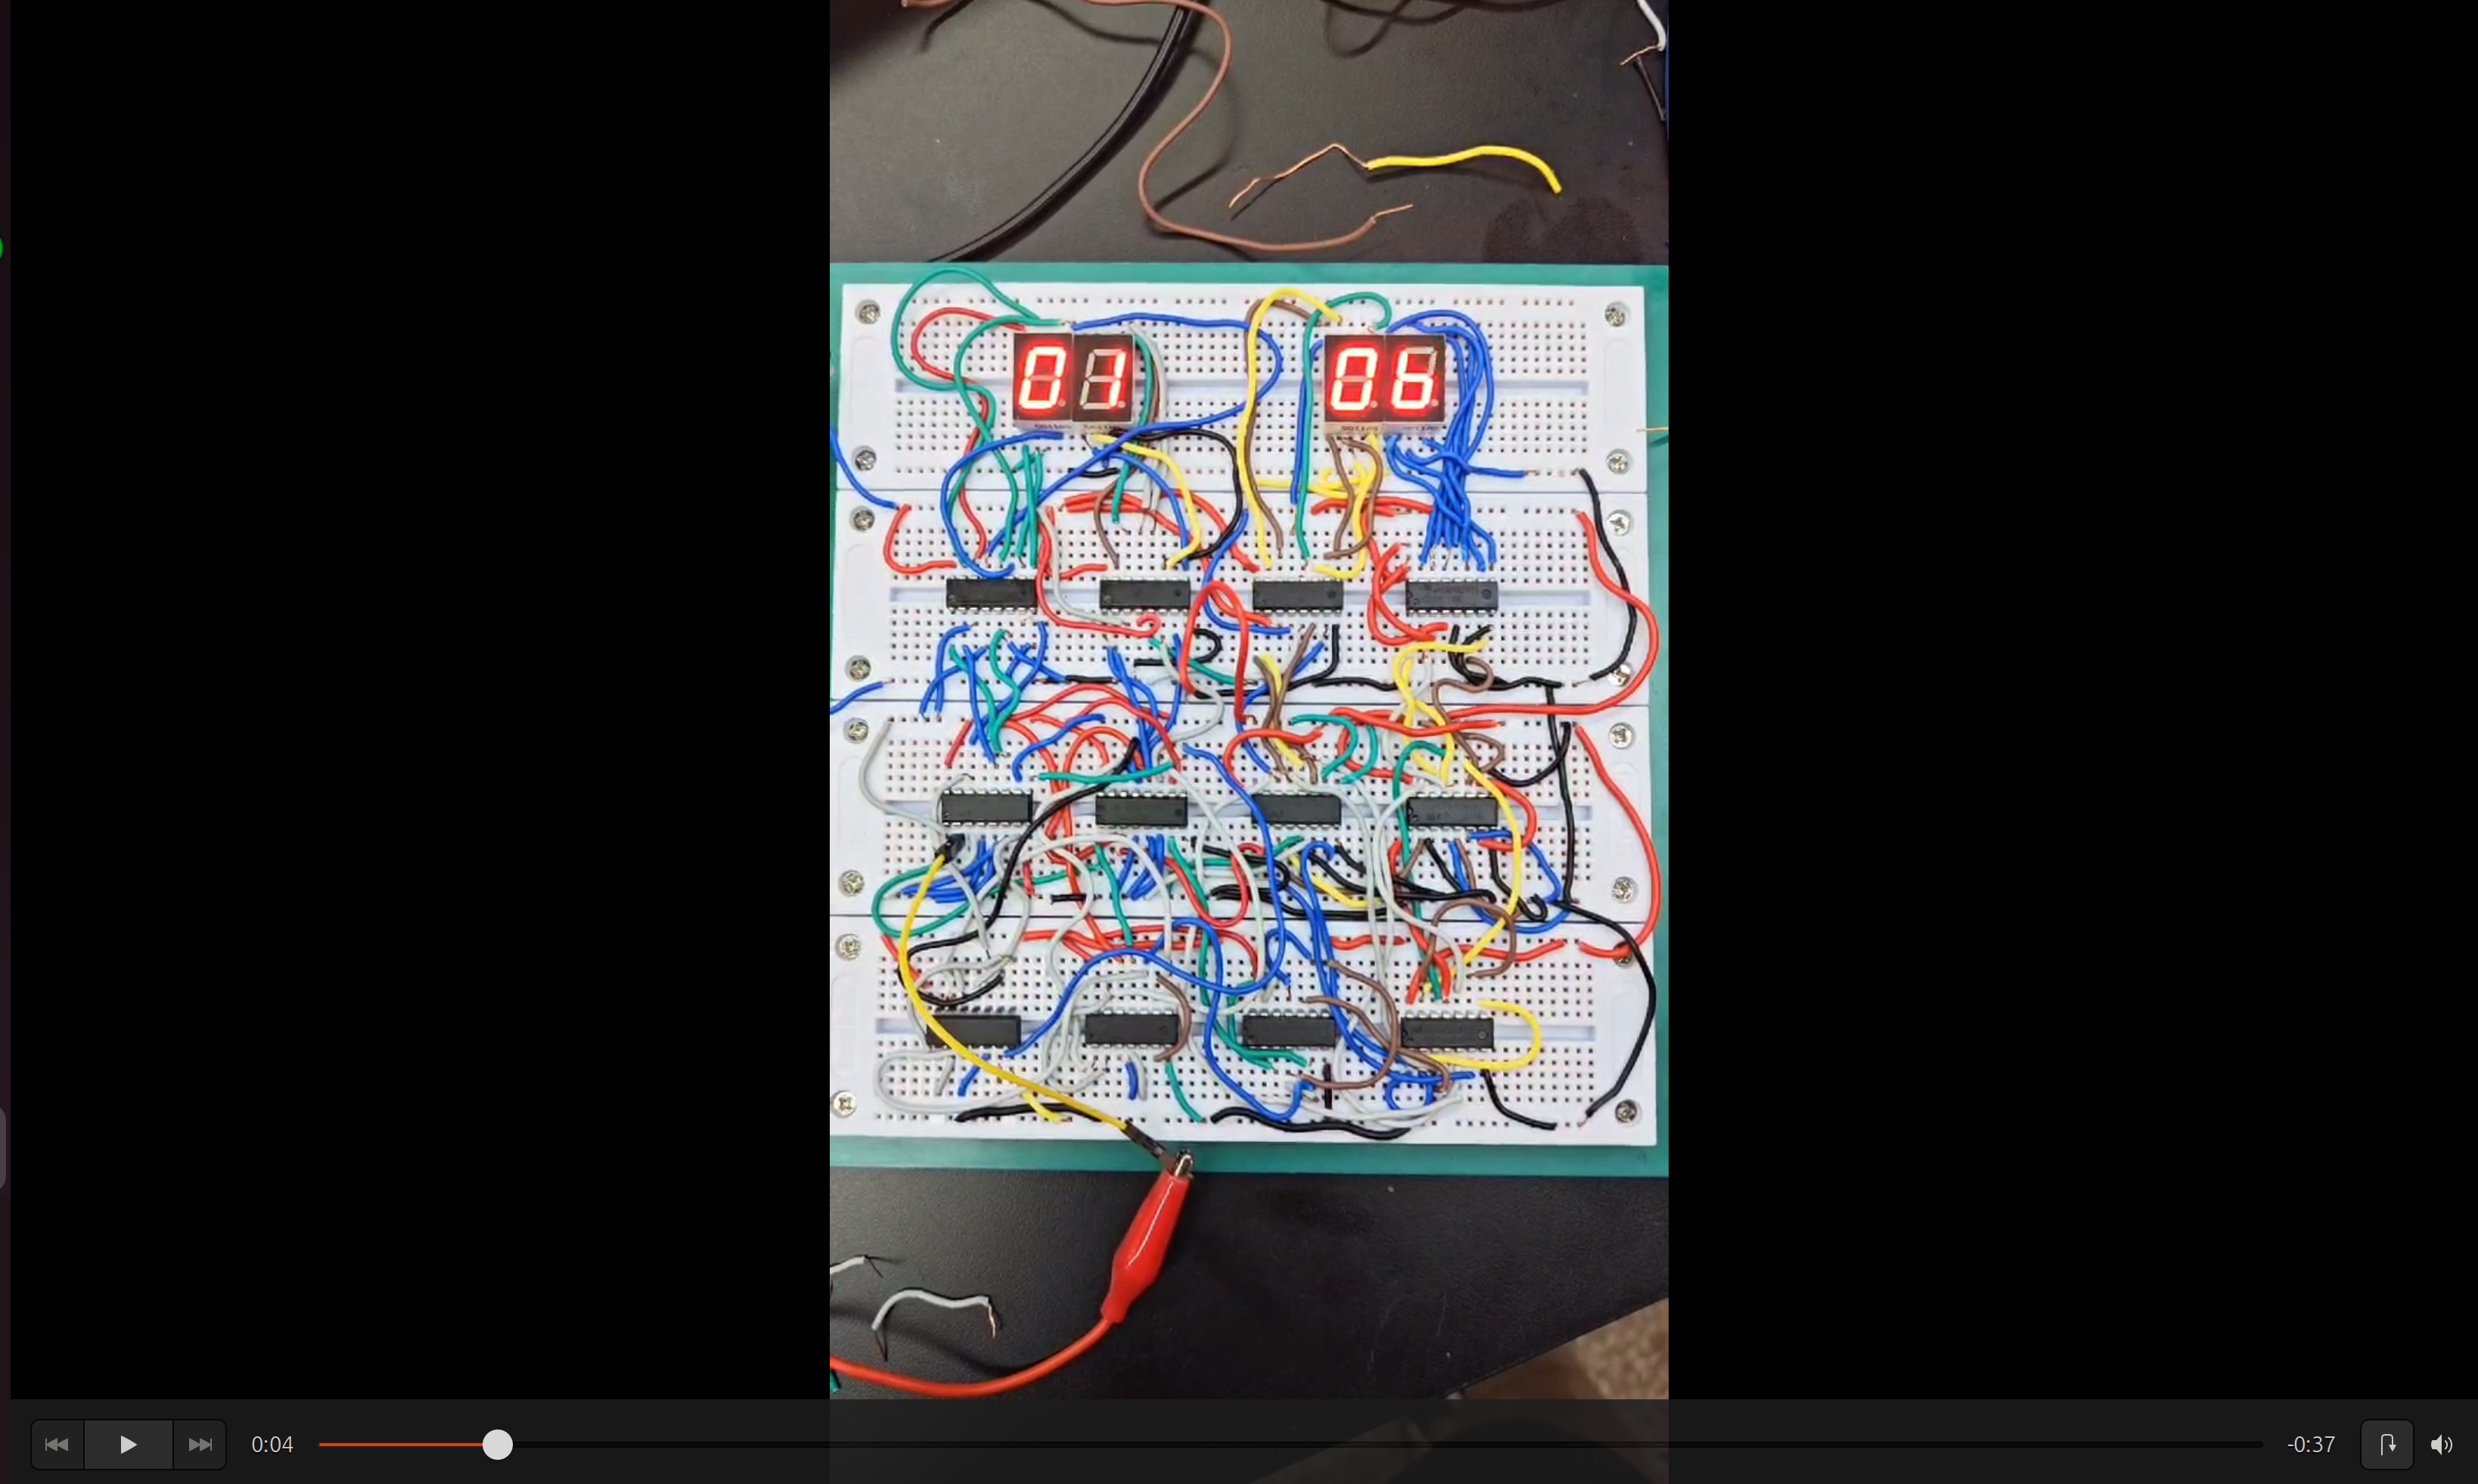
\includegraphics[width=0.86\textwidth]{figures/oscilloscope/image1.png}
    \caption{实验插板实物图}
\end{figure}

实验中上层为数码管，第一层为 CD4511 译码器，第二层为 74HC161 计数器，第三层为 74HC00 与非门。由于实际中没有使用74HC04非门芯片，因此原理图中的74HC04部分由74HC00的与非门实现。

\subsection{翻转过程记录}
\textbf{翻转前：}
\begin{figure}[H]
    \centering
    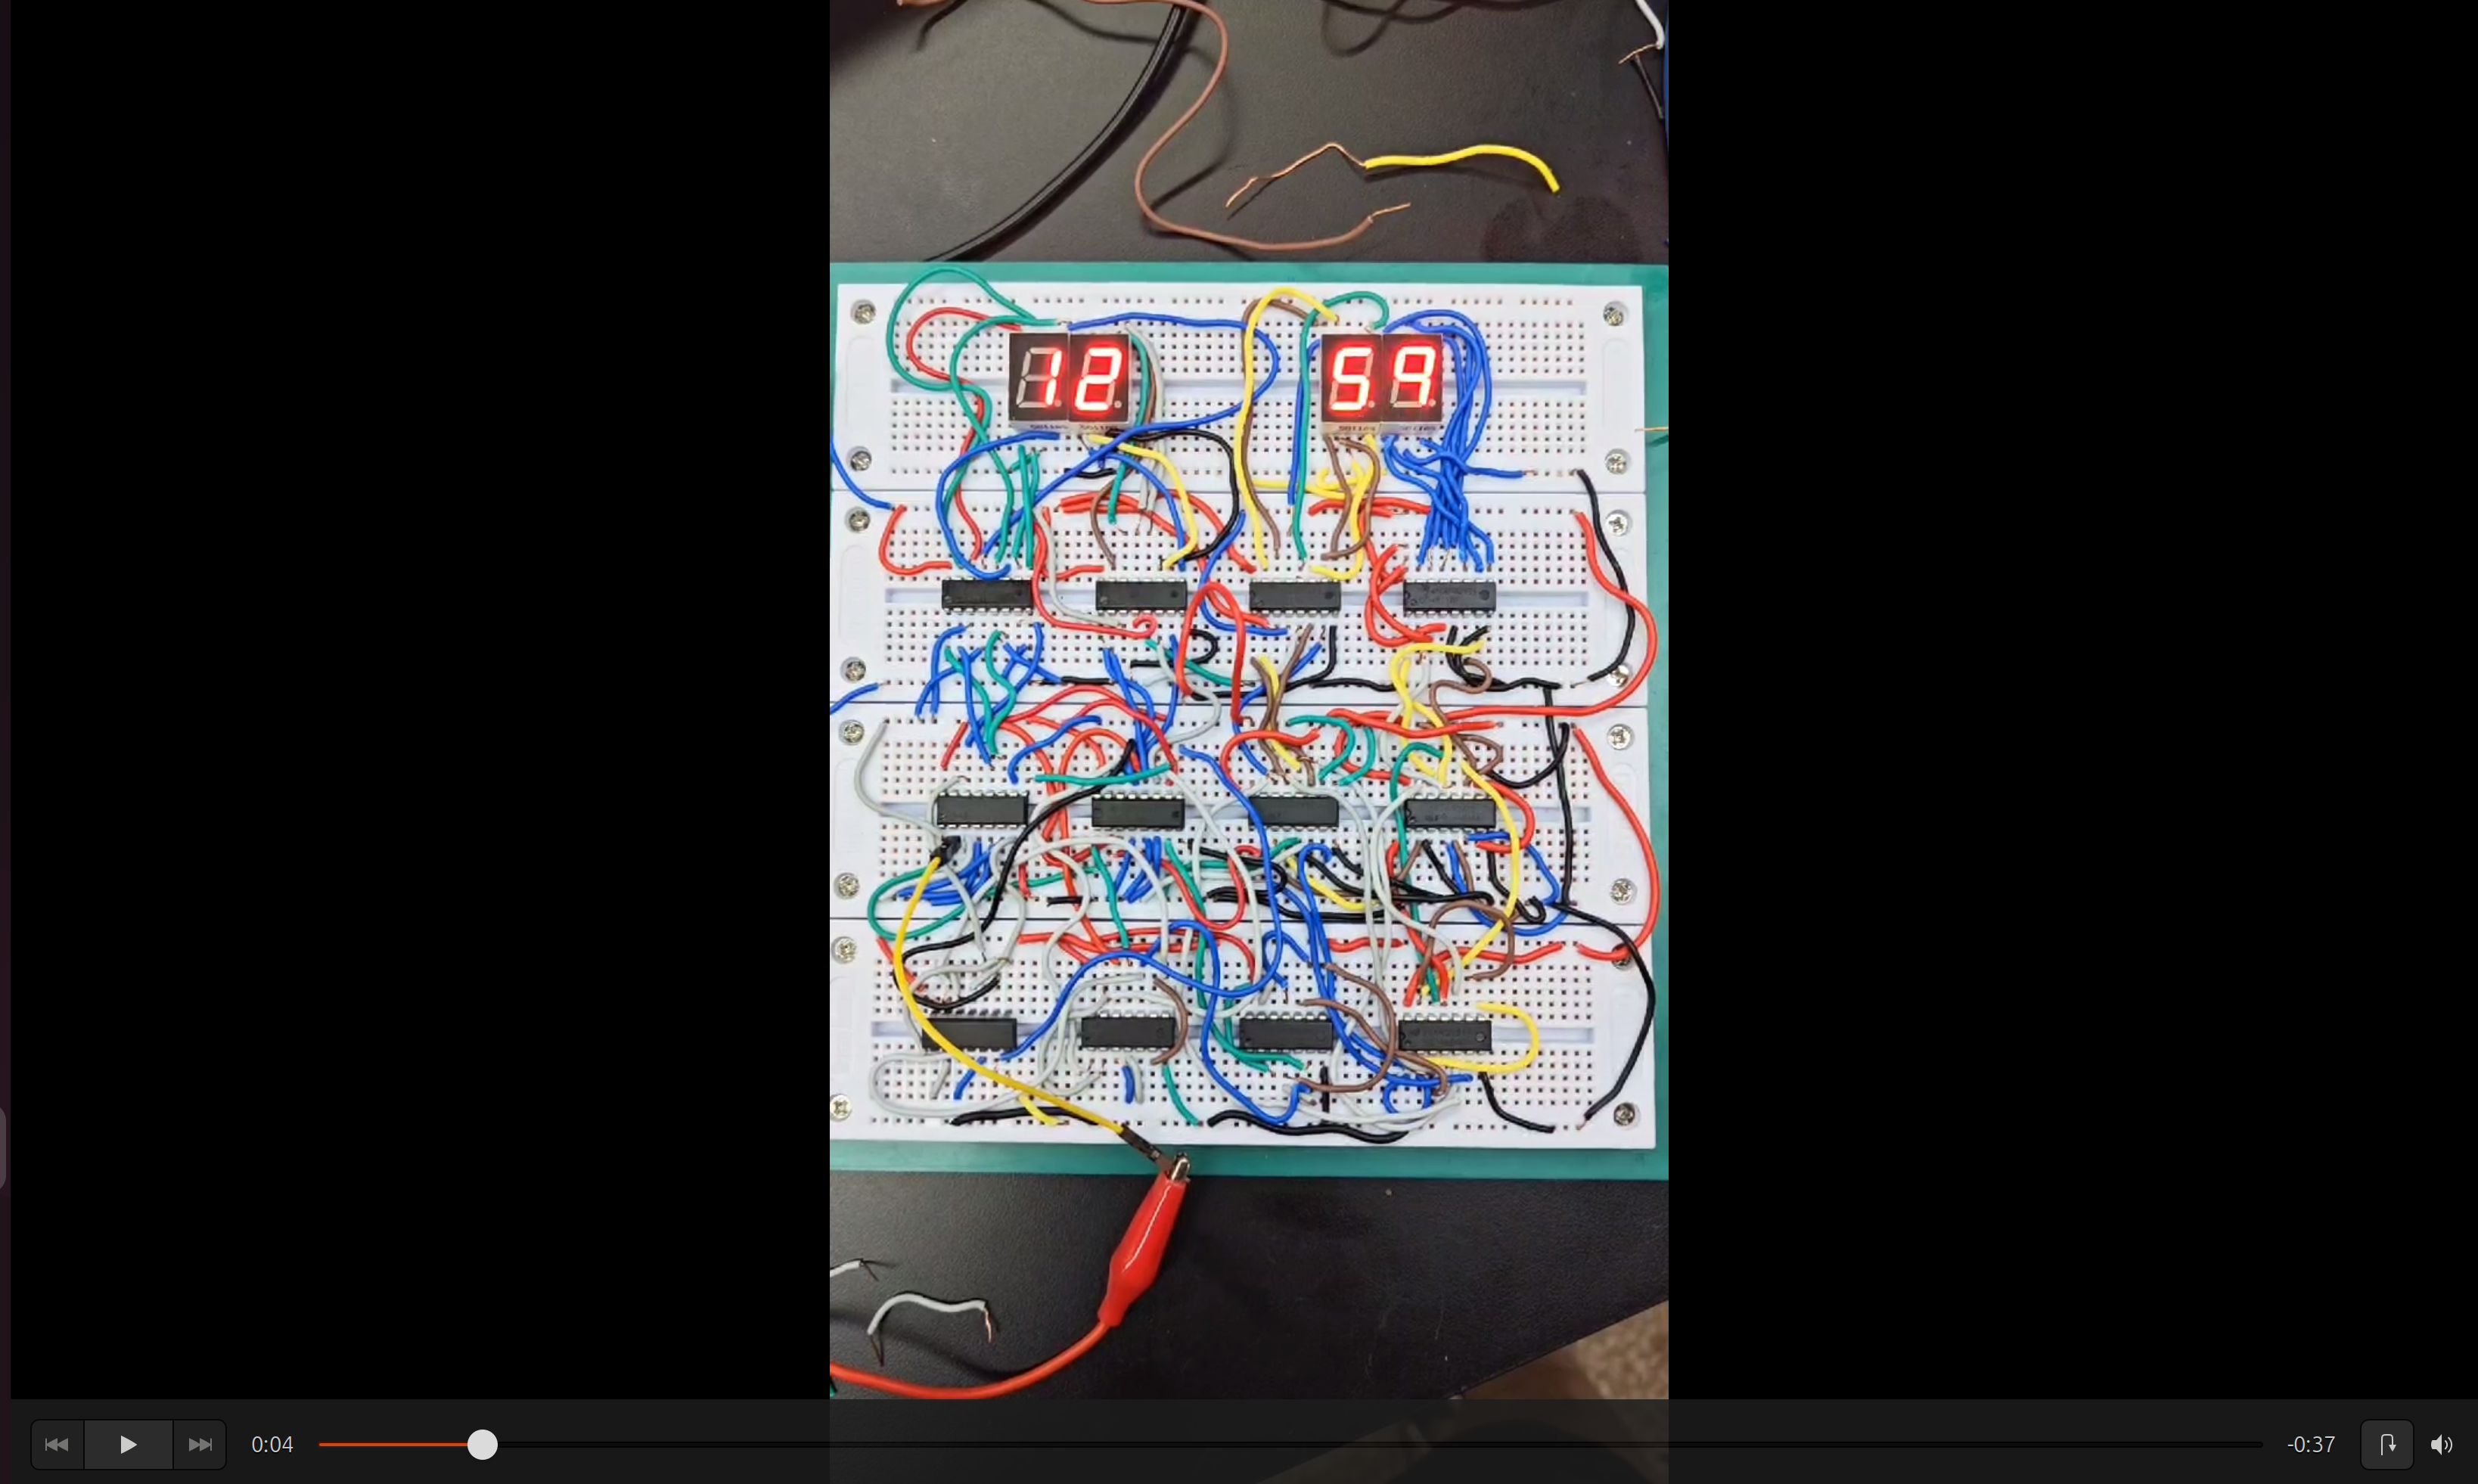
\includegraphics[width=0.85\textwidth]{figures/oscilloscope/image2.png}
    \caption{翻转前显示状态（12时59分）}
\end{figure}

\textbf{翻转后：}
\begin{figure}[H]
    \centering
    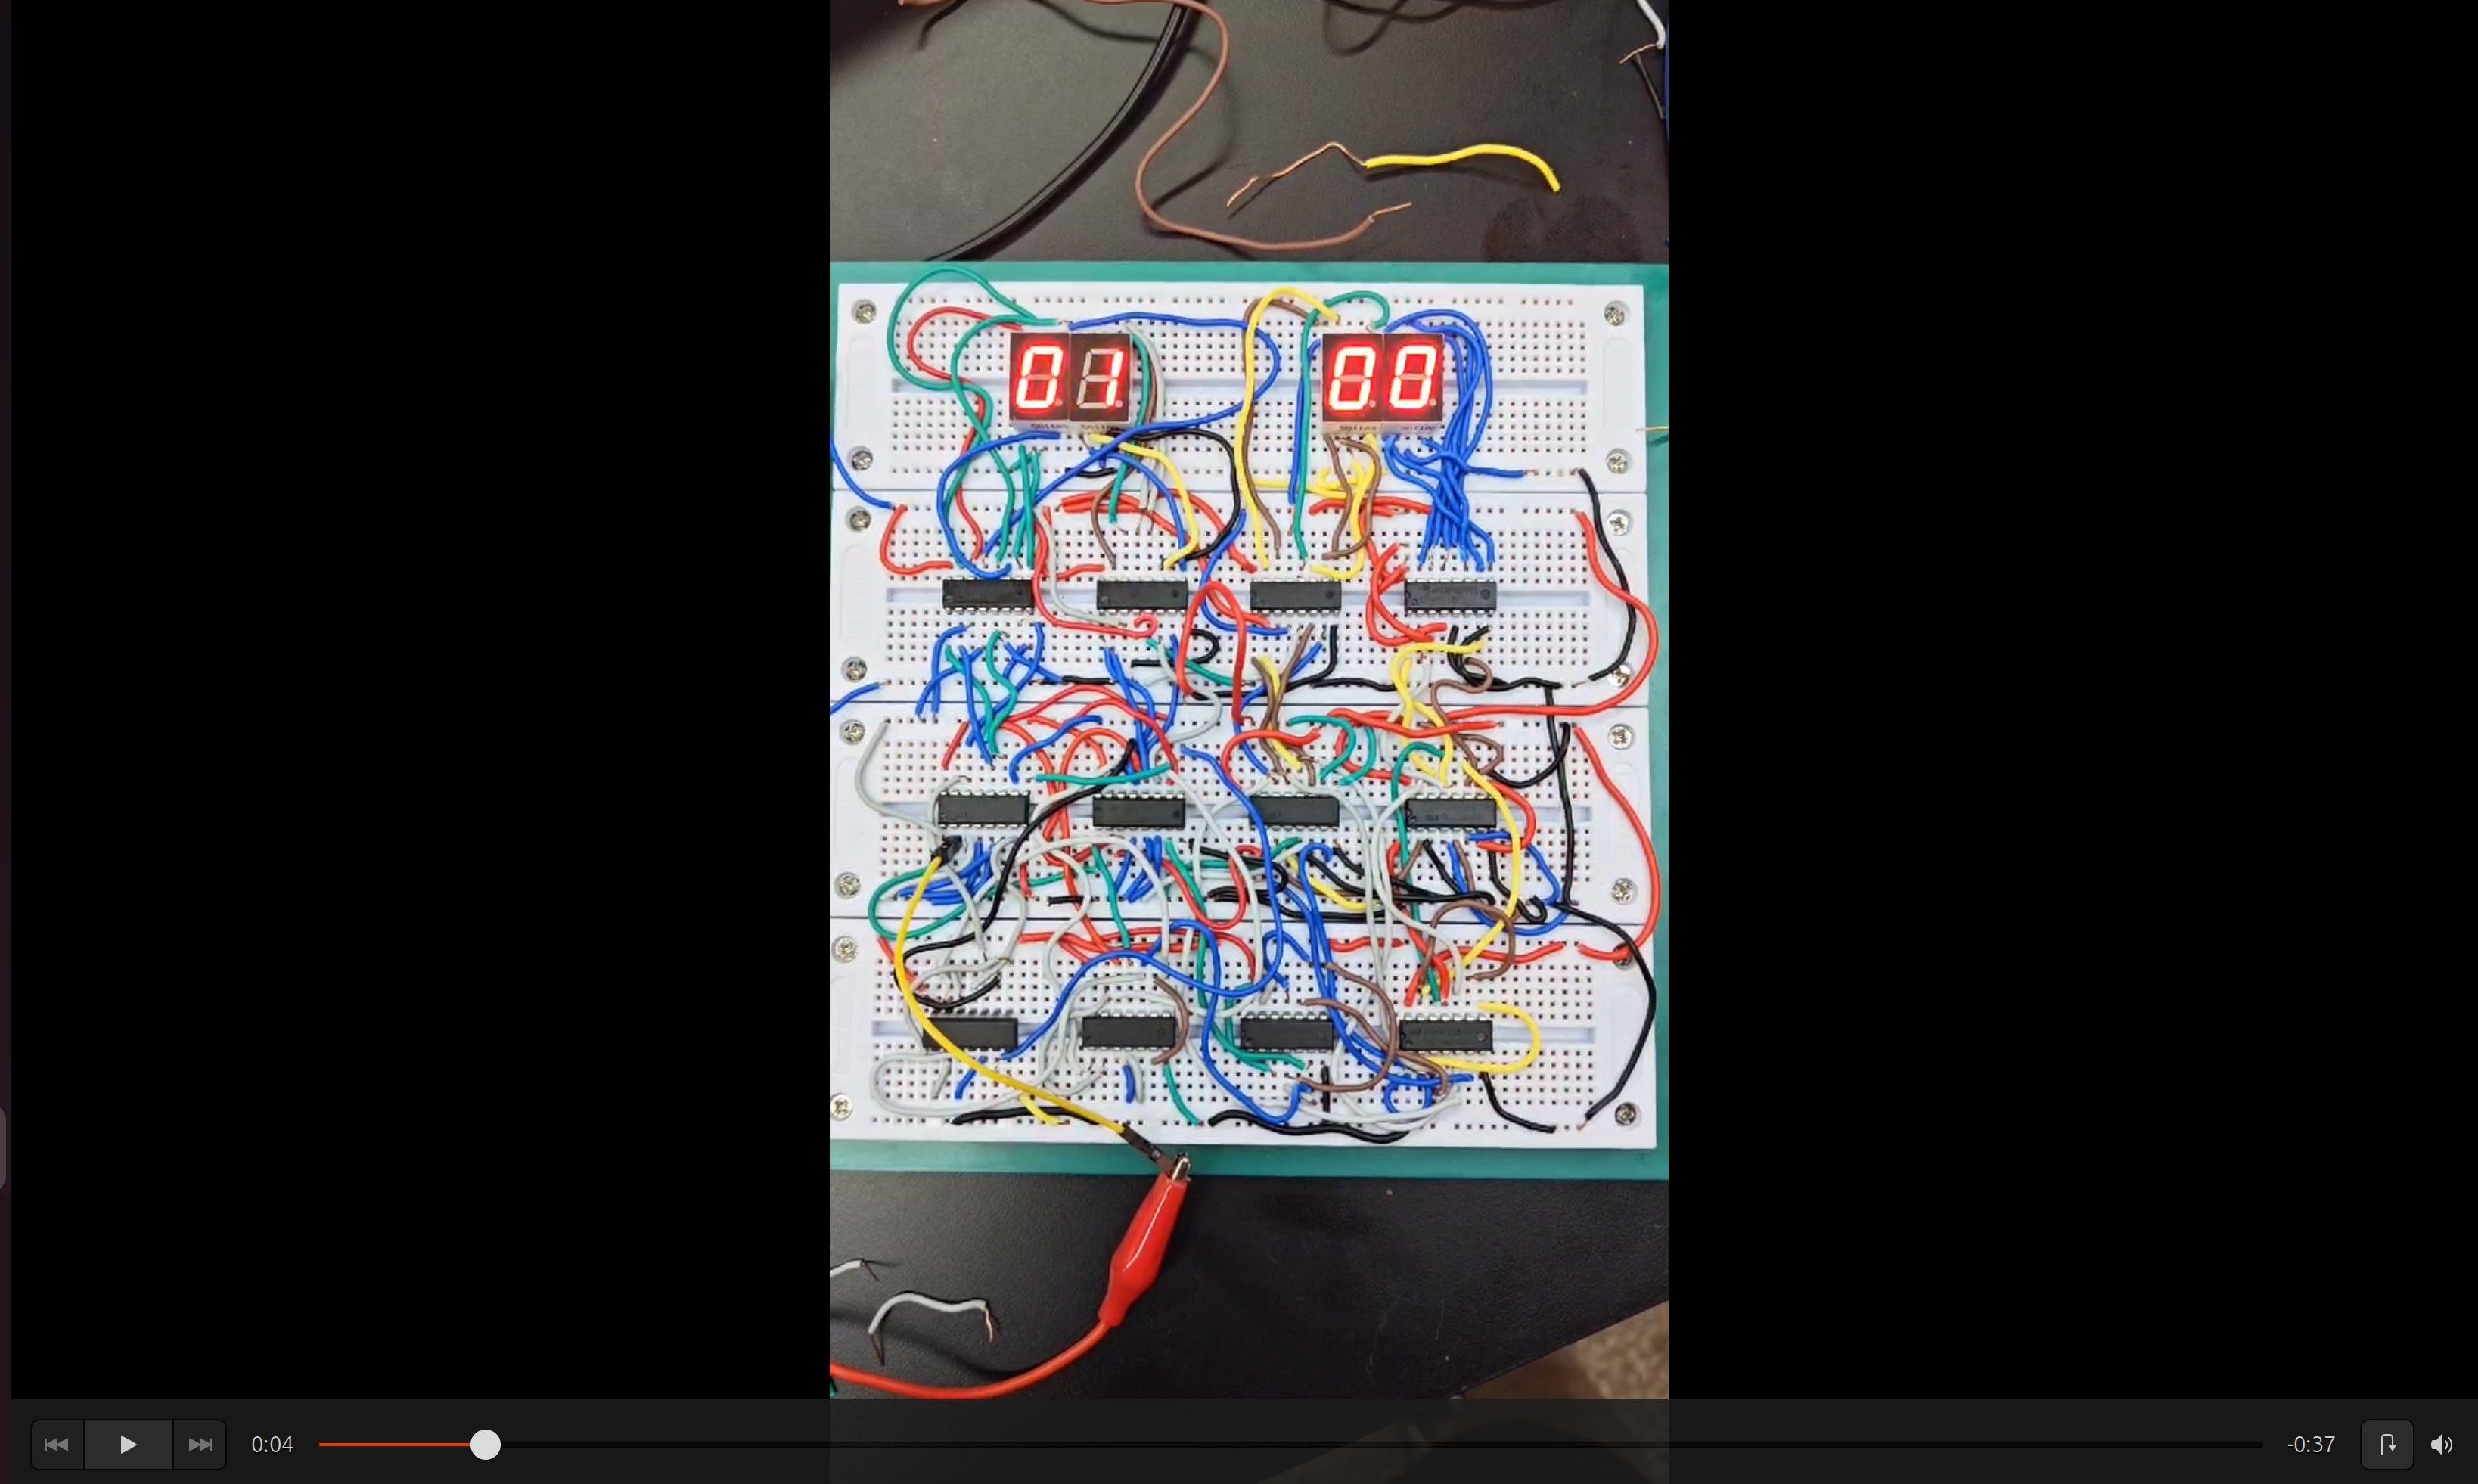
\includegraphics[width=0.85\textwidth]{figures/oscilloscope/image3.png}
    \caption{翻转后显示状态（01时00分）}
\end{figure}

由翻转前后对比可见，计数进位与翻转过程正确，显示功能正常。

\subsection{测量时序波形图}
利用计算机软件绘制出输入 1kHz 正方波时，十进制计数器的 $Q_3,Q_2,Q_1,Q_0$ 波形图如下：
\begin{figure}[H]
    \centering
    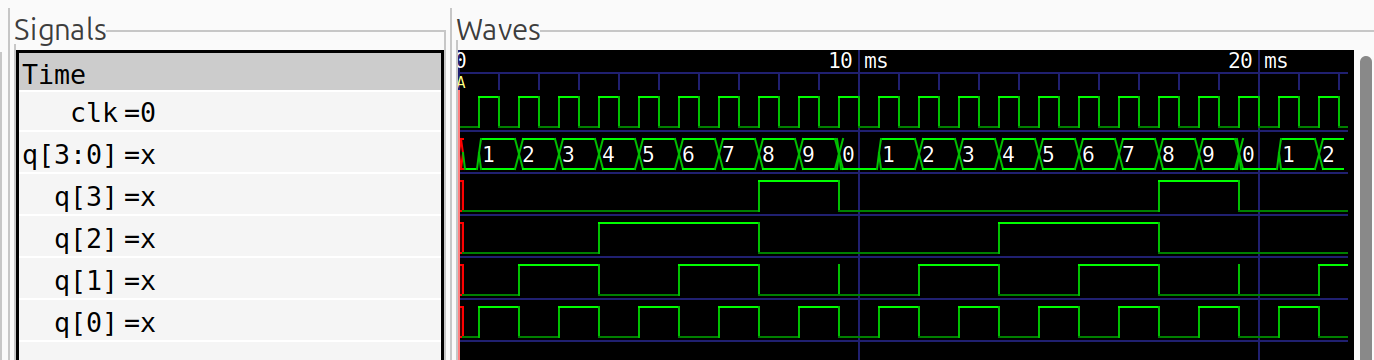
\includegraphics[width=0.64\textwidth]{figures/verilog/image1.png}
    \caption{测量时序波形}
\end{figure}

由波形可见：在 $CP$ 的上升沿到来时，计数器输出按 BCD 码顺序由 $0000$ 递增至 $1001$，对应十进制的 $0\sim9$。当输出继续变化到 $1010$ 时，译码电路产生低电平异步清零信号，使计数器立即回到 $0000$，从而形成十进制循环计数。$Q_0$ 翻转最频繁，$Q_3$ 只在计数到 $8$、$9$ 时为高电平，说明该电路并非完整的四位二进制分频计数，而是经过清零逻辑限制后的 BCD 十进制计数器，波形与理论分析一致。

\subsection{实验结果分析}
输入 1Hz 正方波时，时分数字显示能够每秒更新一次，显示与翻转均正常；输入 1kHz 正方波时，观测到各位输出时序关系符合计数链路预期。说明时钟电路逻辑正确，实验达到目标。

\section{实验中出现的问题、分析及解决方案}
\begin{enumerate}
    \item 数码管显示亮度极低，几乎不可见。\\
    分析：虽然实验推荐将数码管的阴极接$510\Omega$的电阻限流，防止数码管烧毁，但是添加限流电阻后使得数码管电流过低，无法正常显示\\
    解决：直接拆除数码管阴极的限流电阻，改为使用导线直接连接GND，数码管可以以正常亮度显示，且长时间调试未发现数码管存在异常。

    \item 时计时的十位当个位为9时连续进位。\\
    分析：逻辑设计有误，时计时的十位进位不仅应当满足时计时的个位为9，还应当满足分计时为59，才符合正确的计时逻辑。\\
    解决：调整电路逻辑，利用与非门将上述两个逻辑与运算，再将信号传递到时计时的十位使能端，确保时计时显示的正确性。

    \item 初始上电时部分数码管时间错乱或无法显示。\\
    分析：74HC161上电时的初始计数值无法确定，导致初始上电的时间错乱，同时部分74HC161的初始值是$10\sim15$等CD4511认为无效的输入，导致数码管无显示。\\
    解决：将74HC161的CLR端口引出，上电后手动将其置为低电平实现清零，确保计时初值的正确性。
\end{enumerate}

\section{实验总结}
本实验围绕简易数字时钟的设计与调试，完成了计数、译码和数码管显示三部分电路的搭建。计数部分以 $74HC161$ 为核心，通过异步清零方式分别实现分钟个位的模 10 计数和分钟十位的模 6 计数，并利用门电路产生进位信号完成模 60 级联；小时部分在分钟计数达到 $59$ 后产生计数使能信号，实现小时计数的正确递增，并通过译码逻辑完成 $12$ 时 $59$ 分到 $01$ 时 $00$ 分的翻转。显示部分利用 CD4511 将计数器输出的 BCD 码转换为七段数码管显示信号，使计时结果能够直观显示。

通过本次实验，进一步理解了中规模集成计数器的使能、进位、清零和级联方法，也体会到时序电路设计中状态译码与控制信号时序的重要性。实验不仅验证了数字时钟的基本逻辑功能，也提高了对复杂组合逻辑和时序逻辑混合电路的分析、排错与系统联调能力。

\end{document}
